\documentclass[preprint,12pt,aps,pra,showkeys,amsmath,amssymb,superscriptaddress,floatfix]{revtex4-2}
\usepackage[T1]{fontenc}
\usepackage[utf8]{inputenc}
\usepackage{amsmath,amssymb,amsthm,mathtools,mathrsfs}
\usepackage{microtype,booktabs,enumitem}
\usepackage{xcolor,tikz,etoolbox}
\usepackage[skins,breakable]{tcolorbox}
\usepackage{needspace}
% Keep diagram geometry independent of REVTeX preprint body spacing.
\AtBeginEnvironment{tikzpicture}{\linespread{1}\selectfont}
\usetikzlibrary{arrows.meta,positioning,calc,fit,decorations.pathreplacing}
\usepackage{graphicx}
\usepackage{hyperref}

\definecolor{MMBlue}{RGB}{0,82,155}
\definecolor{MMOrange}{RGB}{200,80,0}
\tikzset{
 mmnode/.style={draw=MMBlue,rounded corners=2pt,fill=MMBlue!4,align=left,execute at begin node={\raggedright},text width=5cm,font=\fontsize{10}{12}\selectfont,inner sep=6pt},
 mmimport/.style={mmnode,draw=black!65,fill=black!4},
 mmcandidate/.style={mmnode,draw=MMOrange,dashed,fill=MMOrange!5},
 mmrejected/.style={mmnode,draw=black,densely dotted,fill=black!8},
 mmproof/.style={->,thick,MMBlue},
 mmflow/.style={->,semithick,black!70},
 mmrepair/.style={->,dashed,thick,MMOrange},
 mmcandidatearrow/.style={->,dashed,semithick,MMOrange},
 mmnote/.style={font=\scriptsize,fill=white,inner sep=2pt,align=center}}

\usepackage[section]{placeins}
\setlength{\emergencystretch}{3em}
\setlist{itemsep=3pt,topsep=4pt}
\newtheorem{theorem}{Theorem}[section]
\newtheorem{proposition}[theorem]{Proposition}
\newtheorem{lemma}[theorem]{Lemma}
\newtheorem{corollary}[theorem]{Corollary}
\theoremstyle{definition}
\newtheorem{definition}[theorem]{Definition}
\newtheorem{example}[theorem]{Example}
\theoremstyle{remark}
\newtheorem{remark}[theorem]{Remark}
% Avoid isolated statement headings and single-line paragraph fragments.
\BeforeBeginEnvironment{theorem}{\Needspace{6\baselineskip}}
\BeforeBeginEnvironment{definition}{\Needspace{5\baselineskip}}
\BeforeBeginEnvironment{proposition}{\Needspace{5\baselineskip}}
\BeforeBeginEnvironment{lemma}{\Needspace{5\baselineskip}}
\BeforeBeginEnvironment{corollary}{\Needspace{5\baselineskip}}
\clubpenalty=5000
\widowpenalty=5000
\newcommand{\R}{\mathbb R}\newcommand{\Z}{\mathbb Z}\newcommand{\N}{\mathbb N}
\newcommand{\Pa}{\operatorname{Pa}}\newcommand{\Desc}{\operatorname{Desc}}
\newcommand{\cl}{\operatorname{cl}}\newcommand{\cost}{\operatorname{cost}}
\newcommand{\status}{\operatorname{status}}
% Faculty cards: a visual rail groups the five faculties within one agent.
% The rail has no arrowhead and does not represent a proof dependency.
\newcommand{\mmfacultybadge}[1]{%
 \node[circle,draw=MMBlue,line width=1pt,fill=white,
 minimum size=7mm,inner sep=0pt,font=\sffamily\small\bfseries,text=MMBlue]
 at ([xshift=15pt,yshift=-15pt]frame.north west) {#1};}
\newcommand{\mmfacultyrail}{%
 \draw[MMBlue!80,line width=1pt]
 ([xshift=15pt,yshift=2pt]frame.north west)--
 ([xshift=15pt,yshift=-2pt]frame.south west);}
\newtcolorbox{mmfacultybox}[2]{enhanced,breakable,
 colback=MMBlue!4,colframe=MMBlue!4,boxrule=0pt,arc=3pt,
 left=39pt,right=9pt,top=4pt,bottom=4pt,
 before skip=2pt,after skip=2pt,
 fontupper=\small\linespread{1.1}\selectfont,
 overlay unbroken={\mmfacultyrail\mmfacultybadge{#1}},
 overlay first={\mmfacultyrail\mmfacultybadge{#1}},
 overlay middle={\mmfacultyrail},overlay last={\mmfacultyrail}}
\newcommand{\mmfaculty}[3]{%
 \begin{mmfacultybox}{#1}{#2}
 {\sffamily\bfseries\color{MMBlue}#2}\par\smallskip #3
 \end{mmfacultybox}}
\newcommand{\agent}[9]{%
 \Needspace{8\baselineskip}
 \subsubsection{#1}
 \noindent\textbf{Object.} #2\par
 \noindent\textbf{Role.} #3\par\smallskip
 \mmfaculty{E}{Ego}{#4}
 \mmfaculty{M}{Memory}{#5}
 \mmfaculty{I}{Intellect}{#6}
 \mmfaculty{S}{Sense}{#7}
 \mmfaculty{A}{Action}{#8}
 \smallskip\noindent #9\par}

\usepackage{longtable,array,calc}
\providecommand{\tightlist}{\setlength{\itemsep}{2pt}\setlength{\parskip}{0pt}}
\makeatletter
\def\frontmatter@abstract@produce{\par\addvspace{\frontmatter@preabstractspace}%
\begingroup\prep@absbox\unvbox\absbox\post@absbox\endgroup
\addvspace{\frontmatter@postabstractspace}}
\makeatother
\newcommand{\field}[2]{\par\smallskip\noindent\textbf{#1.} #2\par}
\setlength{\emergencystretch}{5em}
\AtBeginEnvironment{verbatim}{\small\linespread{1.0}\selectfont}


\hypersetup{colorlinks=true,linkcolor=MMBlue,urlcolor=MMBlue,pdfauthor={Dibakar Sigdel}}

\begin{document}

\title{Strong Nullstellensatz via Rabinowitsch's Trick\\[4pt]\large An End-to-End Meta-Math Walkthrough}

\author{Dibakar Sigdel}

\affiliation{Mindverse Computing LLC, Lynnwood, WA 98087, USA}

\date{October 2026}

\begin{abstract}

Turn the assertion that a polynomial never becomes nonzero on the
variety into an inconsistent system by adjoining an inverse variable.
The report presents the target theorem, declared imports, a dependency
graph, five-faculty node contracts, a continuous proof, a worked
example, and a hypothesis-repair audit. It is an authored mathematical
exposition, not a deployed-agent transcript or a formal proof-assistant
certificate.

\end{abstract}\maketitle\linespread{1.12}\selectfont

\noindent\textbf{AG-03 / Algebraic Geometry / Report v1}

\section{Target and import contract}

\begin{theorem}

For an algebraically closed field \(k\), finite \(n\), and any ideal
\(I\subset k[x_1,\ldots,x_n]\), prove \(I(V(I))=\sqrt I\). Here \(I(S)\)
is the ideal of polynomials vanishing on \(S\), and
\(\sqrt I=\{f:f^m\in I\text{ for some integer }m\ge1\}\).

\end{theorem}

\subsection{Foundations and permitted imports}

Import AG-02 in the following exact form: a proper ideal in a
finite-variable polynomial ring over algebraically closed \(k\) has a
common zero. Use localization at the powers of a nonzero polynomial and
finite ideal-combination identities. No effective bound on the exponent
is assumed or concluded.

\clearpage\section{Node interaction workflow}

\begin{center}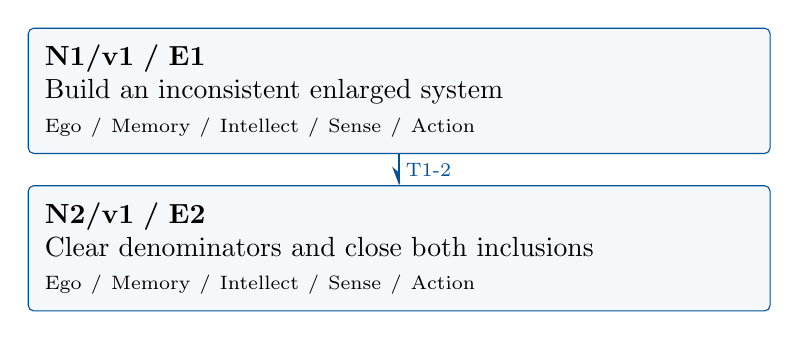
\begin{tikzpicture}[>=Stealth,x=1cm,y=1cm]

\node[mmnode,text width=9cm,minimum height=1.25cm] (N1) at (0,0.0) {\textbf{N1/v1 / E1}\\Build an inconsistent enlarged system\\{\scriptsize Ego / Memory / Intellect / Sense / Action}};

\node[mmnode,text width=9cm,minimum height=1.25cm] (N2) at (0,-2.0) {\textbf{N2/v1 / E2}\\Clear denominators and close both inclusions\\{\scriptsize Ego / Memory / Intellect / Sense / Action}};

\draw[mmproof] (N1.south) -- node[mmnote,right] {T1-2} (N2.north);

\end{tikzpicture}\end{center}

Each box is one mathematical agent containing all five faculties. Blue
arrows carry the versioned exports listed below. The layout gives a
reading order; only drawn arrows assert dependencies. Diagnostic repair
is separate from the proof DAG.

\subsection{Versioned evidence-transfer ledger}

\begingroup\small\linespread{1.05}\selectfont

\Needspace{5\baselineskip}\field{T1-2: N1/E1/v1 to N2}{\(1\in J\), so \(1=\sum_{j=1}^s A_j(x,y)g_j(x)+B(x,y)(1-yf(x))\) for
finitely many \(g_j\in I\).}

\field{Receiving activity}{N2.1}

\field{Compatibility}{E1/v1; \(f\ne0\) for the localization step, with \(f=0\) treated
separately. Check: Zero cannot be inverted, and the exponent clearing
all denominators must be chosen for the finite entire sum.}

\endgroup

\clearpage\section{Agent roles and five-faculty activities}\begingroup\small\linespread{1.05}\selectfont\setlist{itemsep=1pt,topsep=2pt}

\subsection{N1/v1: Build an inconsistent enlarged system}

\field{Object and role}{Combine vanishing of \(f\) on the original zeros with the equation that
would make it invertible. \textbf{Local obligation:} \(1\in J\), so
\(1=\sum_{j=1}^s A_j(x,y)g_j(x)+B(x,y)(1-yf(x))\) for finitely many
\(g_j\in I\).}

\field{Inputs}{\(f\in I(V(I))\) and the ideal \(J=(I,1-yf)\) in
\(k[x_1,\ldots,x_n,y]\).}

\mmfaculty{E}{Ego}{Publish E1/v1 only after establishing this obligation: \(1\in J\), so
\(1=\sum_{j=1}^s A_j(x,y)g_j(x)+B(x,y)(1-yf(x))\) for finitely many
\(g_j\in I\).}

\mmfaculty{M}{Memory}{\(f\in I(V(I))\) and the ideal \(J=(I,1-yf)\) in
\(k[x_1,\ldots,x_n,y]\). Retain the stated assumptions and import
versions.}

\mmfaculty{I}{Intellect}{Combine vanishing of \(f\) on the original zeros with the equation that
would make it invertible.}

\mmfaculty{S}{Sense}{The new variable \(y\) is independent; the weak Nullstellensatz applies
in \(n+1\) variables over the same algebraically closed field.}

\mmfaculty{A}{Action}{Carry out activities N1.1--N1.2 below, retaining each calculation and
construction as evidence.}

\smallskip\noindent\textbf{Numbered mathematical activities}

\begin{enumerate}[label=N1.\arabic*,leftmargin=3.4em]

\item A common zero \((a,b)\) of \(J\) would satisfy \(a\in V(I)\), hence
\(f(a)=0\), while also \(1-bf(a)=0\). This would give \(1=0\), so \(J\)
has no common zero.

\item By the contrapositive of AG-02, \(J\) is the whole ring. Membership of
\(1\) in the generated ideal means exactly a finite
polynomial-combination identity of the displayed form; finite generation
of all of \(I\) is not required for this individual identity.

\end{enumerate}

\field{Export E1/v1}{\(1\in J\), so \(1=\sum_{j=1}^s A_j(x,y)g_j(x)+B(x,y)(1-yf(x))\) for
finitely many \(g_j\in I\).}

\field{Acceptance gate}{The new variable \(y\) is independent; the weak Nullstellensatz applies
in \(n+1\) variables over the same algebraically closed field.}

\field{Targeted repair}{If inconsistency is equated with the unit ideal over an arbitrary field,
restore the algebraic-closure hypothesis before invoking AG-02. Withhold
this export and recheck its descendants after a versioned correction.}

\clearpage

\subsection{N2/v1: Clear denominators and close both inclusions}

\field{Object and role}{Substitute \(y=f^{-1}\), multiply by a sufficiently large power of
\(f\), and prove the converse directly. \textbf{Local obligation:}
\(I(V(I))=\sqrt I\).}

\field{Inputs}{E1/v1; \(f\ne0\) for the localization step, with \(f=0\) treated
separately. Incoming proof exports: E1/v1 at N2.1.}

\mmfaculty{E}{Ego}{Publish E2/v1 only after establishing this obligation:
\(I(V(I))=\sqrt I\).}

\mmfaculty{M}{Memory}{E1/v1; \(f\ne0\) for the localization step, with \(f=0\) treated
separately. Incoming proof exports: E1/v1 at N2.1. Retain the stated
assumptions and import versions.}

\mmfaculty{I}{Intellect}{Substitute \(y=f^{-1}\), multiply by a sufficiently large power of
\(f\), and prove the converse directly.}

\mmfaculty{S}{Sense}{Zero cannot be inverted, and the exponent clearing all denominators must
be chosen for the finite entire sum.}

\mmfaculty{A}{Action}{Carry out activities N2.1--N2.2 below, retaining each calculation and
construction as evidence.}

\smallskip\noindent\textbf{Numbered mathematical activities}

\begin{enumerate}[label=N2.\arabic*,leftmargin=3.4em]

\item If \(f=0\), it is already in \(\sqrt I\). Otherwise evaluate the E1
identity in \(k[x_1,\ldots,x_n,1/f]\) at \(y=1/f\). The last term
vanishes, leaving \(1=\sum_j A_j(x,1/f)g_j(x)\).

\item Choose \(m\ge1\) at least the largest \(y\)-degree of the finitely many
\(A_j\). Multiplication by \(f^m\) yields \(f^m=\sum_j h_j(x)g_j(x)\)
with polynomial \(h_j\), so \(f\in\sqrt I\). Conversely, if \(f^m\in I\)
and \(a\in V(I)\), then \(f(a)^m=0\) in the field \(k\), hence
\(f(a)=0\). This proves both inclusions, including \(I\) equal to the
unit ideal.

\end{enumerate}

\field{Export E2/v1}{\(I(V(I))=\sqrt I\).}

\field{Acceptance gate}{Zero cannot be inverted, and the exponent clearing all denominators must
be chosen for the finite entire sum.}

\field{Targeted repair}{If the conclusion is \(f\in I\) rather than \(f^m\in I\), retain the
denominator-clearing exponent; discarding it loses multiplicity
information. Withhold this export and recheck its descendants after a
versioned correction.}

\endgroup\clearpage\section{Continuous mathematical proof}\label{sec:proof}

\subsection{N1 --- Build an inconsistent enlarged
system}\label{n1-build-an-inconsistent-enlarged-system}

\begin{enumerate}
\def\labelenumi{\arabic{enumi}.}
\item
  \textbf{N1.1.} A common zero \((a,b)\) of \(J\) would satisfy
  \(a\in V(I)\), hence \(f(a)=0\), while also \(1-bf(a)=0\). This would
  give \(1=0\), so \(J\) has no common zero.
\item
  \textbf{N1.2.} By the contrapositive of AG-02, \(J\) is the whole
  ring. Membership of \(1\) in the generated ideal means exactly a
  finite polynomial-combination identity of the displayed form; finite
  generation of all of \(I\) is not required for this individual
  identity.
\end{enumerate}

\subsection{N2 --- Clear denominators and close both
inclusions}\label{n2-clear-denominators-and-close-both-inclusions}

\begin{enumerate}
\def\labelenumi{\arabic{enumi}.}
\item
  \textbf{N2.1.} If \(f=0\), it is already in \(\sqrt I\). Otherwise
  evaluate the E1 identity in \(k[x_1,\ldots,x_n,1/f]\) at \(y=1/f\).
  The last term vanishes, leaving \(1=\sum_j A_j(x,1/f)g_j(x)\).
\item
  \textbf{N2.2.} Choose \(m\ge1\) at least the largest \(y\)-degree of
  the finitely many \(A_j\). Multiplication by \(f^m\) yields
  \(f^m=\sum_j h_j(x)g_j(x)\) with polynomial \(h_j\), so
  \(f\in\sqrt I\). Conversely, if \(f^m\in I\) and \(a\in V(I)\), then
  \(f(a)^m=0\) in the field \(k\), hence \(f(a)=0\). This proves both
  inclusions, including \(I\) equal to the unit ideal.
\end{enumerate}

\hfill$\square$

\section{Worked orchestration}

For \(I=(x^2,y)\) in \(\mathbb C[x,y]\), \(V(I)=\{(0,0)\}\) and
\(I(V(I))=(x,y)\). The polynomial \(x\) is not in \(I\), but
\(x^2\in I\). The enlarged identity for \(f=x\) is
\(1=(1+tx)(1-tx)+t^2x^2\), illustrating exactly how substitution
\(t=1/x\) recovers the square.

\subsection{Boundary and hypothesis audit}

Over \(\mathbb R\), \(I=(x^2+1)\) has empty real zero set, so
\(I(V(I))=\mathbb R[x]\) while \(\sqrt I=I\). Over an algebraically
closed field the theorem concerns radicals, not equality with arbitrary
nonradical ideals.

\section{Illustrative failure and repair}

The following is an authored diagnostic scenario. Changed assumptions
define a new contract; they do not retroactively prove the original
statement.

\subsection{Rejected argument, diagnosis, and correction}
\textbf{Rejected N2 export:} every polynomial vanishing on \(V(I)\)
belongs to \(I\). The worked example \(x\notin(x^2,y)\) refutes it.
\textbf{Diagnosis:} Action discarded the power introduced when clearing
denominators. \textbf{Repair:} export \(f^m\in I\) and hence
\(f\in\sqrt I\). This narrows the rejected overclaim to the theorem
actually stated in §1; the proof there already includes the correct
exponent.

\subsection{Publication and reuse}
The corrected export retains its explicit assumptions. A hypothetical
revision receives a new version, and each consuming activity is
rechecked; this scenario is not a recorded runtime event. \textbf{Next
direction:} Deduce the inclusion-reversing correspondence between affine
algebraic sets and radical ideals; then compare reduced coordinate rings
with nonreduced schemes.

\par\medskip\begingroup\small\linespread{1.0}\selectfont\noindent\textbf{Provenance.} This authored proof is complete relative to its declared imports. Reuse
each export with its assumptions, proof, and version. The original
Markdown remains available for comparison.
\par\endgroup

\par\smallskip\begingroup\small\linespread{1.0}\selectfont\noindent\textbf{Further reading.} \href{https://www.jmilne.org/math/CourseNotes/ag.html}{J. S. Milne,
Algebraic Geometry}, chapters on commutative algebra, algebraic sets,
and affine varieties; \href{https://www.jmilne.org/math/}{author's
mathematics site}.\par\endgroup

\end{document}
